\iffalse
Oltre alla programmazione logica, PICAT è pensato anche per implementare la programmazione imperativa. Di questa possiede alcuni caratteristiche tipiche come l'assegnazione, oppure costrutti che riguardano il control flow quindi l'if-then-else ed i cicli. 
\fi

\begin{frame}{Programmazione imperativa - 1}

	\begin{columns}
		\begin{column}{0.5\textwidth}
			\begin{itemize}
				\item Assegnazione e side-effects
				\item If-Then-Else
				\item Cicli
				\begin{itemize}
					\item foreach
					\item while
					\item do..while
				\end{itemize}
			\end{itemize}
		\end{column}

		\begin{column}{0.5\textwidth}
			
			\begin{figure}%
				\centering
				\subfigure{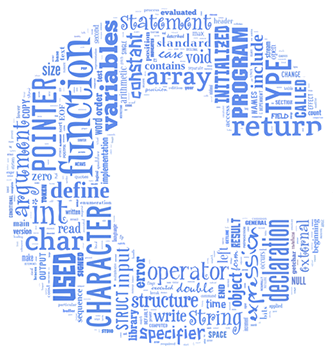
\includegraphics[scale=0.09]{res/cLogo}}\qquad
				\subfigure{
\includegraphics[scale=0.24]{res/c++Logo}}\\
				\subfigure{
\includegraphics[scale=0.03]{res/javaLogo}}%
			\end{figure}

		\end{column}
	\end{columns}

\end{frame}